\section{Introduction}
\paragraph{Objectifs du TP}
\begin{itemize}
	\item {Mesurer avec un oscilloscope le déphasage entre deux tensions évoluant sinusoïdalement dans le temps}
	      
	\item {Calculer la capacité d’un condensateur et l’inductance et la résistance interne d’une bobine}
	      
	\item {Maitriser le mode XY d'un oscilloscope}
\end{itemize}
\paragraph{Matériel:}
\begin{itemize}
	\item {Oscilloscope}
	      
	\item {Générateur de basses fréquences}
	      
	\item {Boîtier Pierron de 4 résistances}
	      
	\item {Support en Plexiglass avec trois résistances identiques R = 100 $\ohm$}
	      
	\item {Condensateur de capacité C = 0,1 $\mu$F}
	      
	\item {Bobine d’inductance L}
	      
	\item {Câbles}
\end{itemize}
\paragraph{Notions théoriques nécessaires à la résolution du problème}
\begin{itemize}
	\item {Nombres complexes}
	      
	\item {Déphasages (temporel et angulaire)}
	      
	\item {Oscilloscope : mesure du déphasage}
\end{itemize}
\subsection{Questions préliminaires}
\subsubsection{Approche théorique : mesure du déphasage en mode XY}
\paragraph{Simulation du fonctionnement de l’oscilloscope en mode XY}
\begin{enumerate}
	\item \textbf{Cas où $\varphi = \pi$ (Opposition de phase)}
	          
	      \begin{minipage}{0.45\textwidth}
	      	\centering
	      	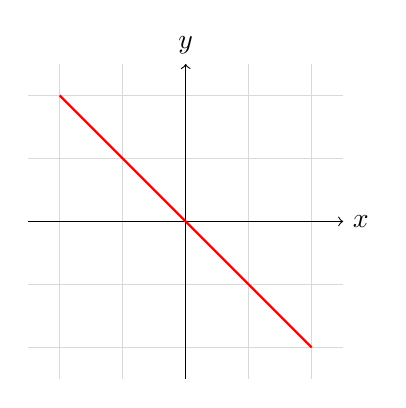
\begin{tikzpicture}[scale=0.8]
	      		\draw[step=1cm,gray!30,very thin] (-2.5,-2.5) grid (2.5,2.5);
	      		\draw[->] (-2.5,0) -- (2.5,0) node[right] {$x$};
	      		\draw[->] (0,-2.5) -- (0,2.5) node[above] {$y$};
	      		\draw[thick, red] (-2,2) -- (2,-2);
	      	\end{tikzpicture}
	      	\captionof{figure}{Courbe pour $\varphi = \pi$}
	      \end{minipage}
	      \hfill
	      \begin{minipage}{0.5\textwidth}
	      	\textbf{Justification :} \\
	      	Si $\varphi = \pi$, alors :
	      	\[ x(t) = U_1 \sin(\omega t + \pi) = -U_1 \sin(\omega t) \]
	      	\[ y(t) = U_2 \sin(\omega t) \]
	      	        
	      	On remarque que $\sin(\omega t) = \frac{y}{U_2}$ et $\sin(\omega t) = -\frac{x}{U_1}$.
	      	En identifiant les deux termes, on obtient l'équation de la trajectoire :
	      	\[ y = -\frac{U_2}{U_1} x \]
	      	        
	      	\textbf{Description :} C'est l'équation d'une droite passant par l'origine avec une pente négative.
	      \end{minipage}
	      
	      \vspace{1cm}
	      \newpage
	\item \textbf{Cas où $\varphi = \pi/2$ (Quadrature de phase)}
	          
	      \begin{minipage}{0.45\textwidth}
	      	\centering
	      	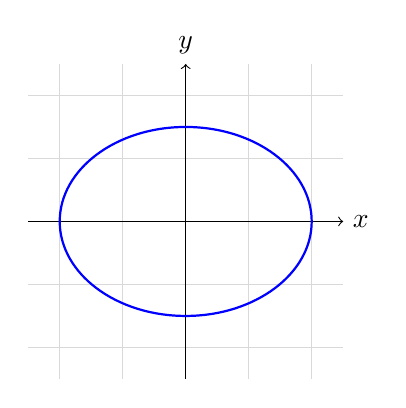
\begin{tikzpicture}[scale=0.8]
	      		\draw[step=1cm,gray!30,very thin] (-2.5,-2.5) grid (2.5,2.5);
	      		\draw[->] (-2.5,0) -- (2.5,0) node[right] {$x$};
	      		\draw[->] (0,-2.5) -- (0,2.5) node[above] {$y$};
	      		\draw[thick, blue] (0,0) ellipse (2cm and 1.5cm);
	      	\end{tikzpicture}
	      	\captionof{figure}{Courbe pour $\varphi = \pi/2$}
	      \end{minipage}
	      \hfill
	      \begin{minipage}{0.5\textwidth}
	      	\textbf{Justification :} \\
	      	Si $\varphi = \pi/2$, alors :
	      	\[ x(t) = U_1 \sin(\omega t + \pi/2) = U_1 \cos(\omega t) \]
	      	\[ y(t) = U_2 \sin(\omega t) \]
	      	        
	      	On utilise la relation trigonométrique $\cos^2(\theta) + \sin^2(\theta) = 1$ :
	      	\[ \left(\frac{x}{U_1}\right)^2 + \left(\frac{y}{U_2}\right)^2 = 1 \]
	      	        
	      	\textbf{Description :} C'est l'équation cartésienne d'une ellipse centrée en $(0,0)$ et dont les axes sont alignés avec ceux de l'oscilloscope. (Si $U_1 = U_2$, c'est un cercle).
	      \end{minipage}
\end{enumerate}
\paragraph{Application : Mesure des déphasages en mode XY} 
$BB'$ représente deux fois l'amplitude de la tension appliquée sur l'axe X donc l'amplitude
du signal $u_{1}(t)$.\\ $D'D$ représente l'amplitude de la tension appliquée sur
l'axe Y donc l'amplitude du signal $u_{2}(t)$.\\ De plus, les longueurs $BB'$ et
$D'D$ ne varient pas avec le déphasage entre les deux signaux. \\ Non, cette
méthode ne permet pas de déterminer si $u_{1}$ est en avance ou en retard. L'ellipse
parcourue dans un sens (avance) ou l'autre (retard) a la même forme sur
l'écran.

\section{Expériences}
\subsection{Expérience n°1 - Circuit RC série }
\subsubsection{Mesure des déphasages entre $u_R(t)$ et $u_G(t)$}
\begin{enumerate}
	\item En observant les courbes en mode DUAL, on constate que la tension
	      $u_{R}(t)$ est en avance par rapport à $u_{G}(t)$. Le décalage temporel $\Delta
	      t$ entre $u_{R}$ et $u_{G}$ est donné par :
	      \[
	      	\Delta t = \frac{\varphi}{\omega}\qquad (\text{avec }\omega = 2\pi f)
	      \]
	      Ainsi, le décalage de phase entre $u_{R}$ et $u_{G}$ vaut :
	      \[
	      	\varphi = 2\pi f\, \Delta t
	      \]
	      \newpage
	      
	\item \leavevmode
	      \begin{center}
	      	\includegraphics[width=0.75\linewidth]{thumbnail_IMG_3767.jpg}
	      	\captionof{figure}{Représentation des courbes $Y_{I}$ et $Y_{II}$ sur l'oscilloscope}
	      	\label{fig:oscillo_YI_YII}
	      \end{center}
	      
	      $Y_{I}$ correspond à la courbe jaune et $Y_{II}$ à la courbe bleue. Les sensibilités
	      verticales sont de $5\,\text{V/div}$ et le balayage horizontal est de $50\,\mu
	      \text{s/div}$.
	      
	      \begin{center}
	      	\includegraphics[width=0.75\linewidth]{thumbnail_IMG_3768.jpg}
	      	\captionof{figure}{Représentation de la courbe de Lissajous en mode XY sur l'oscilloscope}
	      	\label{fig:lissajous}
	      \end{center}
	      Les sensibilités utilisées sont de $5\,\text{V/div}$.
	      \newpage
	          
	\item 
	      D'après la figure 4, l'oscilloscope indique une fréquence d'environ $1,296\,\text{kHz}$, soit $1296\,\text{Hz}$.\\[2mm]
	      Selon les mesures obtenues en mode curseur :
	      \[
	      	\begin{aligned}
	      		\Delta t & = X_2 - X_1                               \\
	      		         & = 502,0\,\mu\text{s} - 388,0\,\mu\text{s} \\
	      		         & \boxed{= 114,0\,\mu\text{s}}              
	      	\end{aligned}
	      \]
	      
	      Ainsi, la période est de :
	      \[
	      	\begin{aligned}
	      		T & = \frac{1}{f}                    \\
	      		  & \approx \frac{1}{1296}           \\
	      		  & \boxed{\approx 772\,\mu\text{s}} 
	      	\end{aligned}
	      \]
	      
	      Enfin, le déphasage de $u_R$ par rapport à $u_G$ est :
	      \[
	      	\boxed{\varphi = \frac{\Delta t}{T} \times 360^\circ \approx 53,2^\circ \approx 0,92~\text{rad}}
	      \]
	\item \textbf{Méthode directe} \\
	      Le décalage temporel se mesure directement sur l'écran de l'oscilloscope. Si le décalage n'occupe qu'une petite portion de l'écran, l'erreur de lecture due à la précision du curseur peut être importante. Ainsi, l'incertitude est relativement élevée.
	      
	      \textbf{Méthode XY} \\
	      Le déphasage se mesure à partir de la forme de l'ellipse. En ajustant les sensibilités horizontales et verticales, on peut agrandir l'ellipse, ce qui permet de mesurer des distances plus grandes et donc plus précises. Ainsi, l'incertitude est plus faible, car l'erreur relative de lecture diminue.
	      
	      On en déduit que la méthode directe est plus simple à réaliser, mais moins précise, contrairement à la méthode XY. Cependant, avec cette dernière, il n'est pas possible de déterminer directement quelle tension est en avance.
\end{enumerate}

\subsubsection{Confrontation expérience-théorie (à faire chez soi)}
\begin{enumerate}
	\item On se place en approximation des régimes quasi-stationnaires. Le circuit est de type RC série (cf. figure 3 dans l'énoncé). On remarque qu'il s'agit d'un pont diviseur de tension. On a donc :
	      \[
	      	Z_R = R
	      \]
	      D'après la formule du diviseur de tension :
	      \[
	      	\begin{aligned}
	      		u_R(t) & = \frac{Z_R}{Z_\text{total}}\, u_G(t) \\
	      		       & \boxed{= \frac{R}{R + Z_C}\, u_G(t)}  
	      	\end{aligned}
	      \]
	      
	\item On passe aux complexes. Ainsi on a $Z_C=\frac{1}{jC\omega}$
	      On a donc :
	      \[
	      	\begin{aligned}
	      		\frac{u_R(t)}{u_G(t)} & = \frac{R}{R + \frac{1}{j C \omega}}   \\
	      		                      & = \frac{1}{1 + \frac{1}{j R C \omega}} 
	      	\end{aligned}
	      \]
	      \[
	      	\boxed{u_R(t) = \frac{1}{1 + \frac{1}{j R C \omega}} \, u_G(t)}
	      \]
	\item Le déphasage $\varphi$ est l'argument du nombre complexe de la fonction de transfert. On pose donc $H = \frac{u_R}{u_G}$.
	      \[
	      	\begin{aligned}
	      		H & = \frac{1}{1+\frac{1}{jRC\omega}}                          \\
	      		  & = \frac{1}{1-j(\frac{1}{RC\omega})} \quad (\frac{1}{j}=-j) 
	      	\end{aligned}
	      \]
	      L'argument d'une fraction est l'argument du numérateur moins celui du dénominateur :
	      \[
	      	\begin{aligned}
	      		\varphi & = \arg(1) - \arg(1 - j \frac{1}{RC\omega})                                          \\
	      		        & = 0 - \arctan(-\frac{1}{RC\omega})                                                  \\
	      		        & = \arctan(\frac{1}{RC\omega})                                                       \\
	      		        & = -(-\arctan(\frac{1}{RC\omega})) \quad \text{(La fonction $\arctan$ est impaire.)} \\
	      		        & \boxed{= \arctan({\frac{1}{RC\omega}})}                                             
	      	\end{aligned}
	      \]
	      Ce signe positif est cohérent avec notre observation expérimentale (cf. figure 3 du compte-rendu). On constate que $u_R$ est en avance sur $u_G$.
	      \newpage
	\item On inverse la relation précédente pour obtenir la capacité C.
	      \[
	      	\begin{aligned}
	      		\tan(\varphi)=\frac{1}{RC\omega} \Rightarrow C=\frac{1}{R\omega\tan(\varphi)} 
	      	\end{aligned}
	      \]
	      Données expérimentales : \\ [1mm]
	      Fréquence $f = 1296\ \text{Hz}$ \\
	      Pulsation $\omega = 2\pi f \approx 8143 \ \text{rad}$ \\
	      Déphasage $\varphi = 53,2^\circ \times \frac{\pi}{180} \approx 0,9285\ \text{rad}$
	      
	      On a donc :
	      \[
	      	\begin{aligned}
	      		C & = \frac{1}{1000 \times 8143 \times \tan(0,9285)} \\
	      		  & \approx 9,18 \times 10^{-8}\ \text{F}            \\
	      		  & \boxed{\approx92\ \text{nF}}                     
	      	\end{aligned}
	      \]
	      Le résultat est cohérent avec la valeur attendue d'un condensateur de $0,1\mu F$. \\
	      Si l'on devait refaire l'expérience, au lieu de se limiter à une seule mesure à une fréquence donnée, il serait mieux de réaliser les mesures pour plusieurs fréquences. Cela permettrait d'étudier la variation du déphasage en fonction de la fréquence.
\end{enumerate}
\subsection{Expérience n°2 - Même circuit mais déphasage entre $u_R$ et $u_C$}
\subsubsection{Manipulation}
\begin{enumerate}
	\setcounter{enumi}{1}
	\item Il est impossible de mesurer directement (c'est-à-dire dans le bon sens) avec ce montage, car l'oscilloscope visualise l'opposé de la tension ($-u_R$). Il faut donc appuyer sur le bouton "inverser", ce qui remettra la tension dans le bon sens.
\end{enumerate}
\subsubsection{Mesures des déphasages}
\begin{table}[h!]
	\centering
	\normalsize
	\renewcommand{\arraystretch}{1.8}
	\begin{tabular}{|c|c|c|c|c|c|c|}
		\hline
		\textbf{Fréquence f (Hz)}                      & 500 & 1000 & 1500 & 2000 & 5000 & 10000 \\
		\hline
		\textbf{Décalage temporel $\Delta T$ ($\mu$s)} & 500 & 260  & 184  & 132  & 58   & 28    \\
		\hline
		\textbf{Déphasage} & 
		$\tfrac{\pi}{2}$ & 
		$\tfrac{13\pi}{25}$ & 
		$\tfrac{69\pi}{125}$ & 
		$\tfrac{66\pi}{125}$ & 
		$\tfrac{29\pi}{50}$ & 
		$\tfrac{14\pi}{25}$ \\
		\hline
	\end{tabular}
	\caption{Mesures des déphasages}
	\label{tab:mesures_dephasages_exp2}
\end{table}
D'après les mesures obtenues, on remarque que le déphasage est quasiment constant lorsque la fréquence varie (il reste proche de $\pi/2$). Contrairement à l'expérience 1, le déphasage ici ne dépend pas de la fréquence.
\newpage
\subsubsection{Confrontation expérience-théorie}
\begin{enumerate}
	\item On utilise la loi d'Ohm. \\
	      Soit $i$ l'intensité traversant le circuit RC série. \\
	      La tension aux bornes de la résistance est :
	      \[
	      	u_R = Ri
	      \]
	      La tension aux bornes du condensateur est :
	      \[
	      	u_C = i Z_C = \frac{1}{j C \omega}\, i
	      \]
	      Le rapport des deux tensions est :
	      \[
	      	\begin{aligned}
	      		\frac{u_R}{u_C} & = \frac{Ri}{\frac{1}{jC\omega}i} \\
	      		                & = j R C \omega                   
	      	\end{aligned}
	      \]
	      \[
	      	\boxed{\frac{u_R}{u_C} = j R C \omega}
	      \]
	      On retombe ainsi sur l'équation 19 de l'énoncé. Puisque $\frac{\pi}{2}$ est une constante, il ne contient pas le terme $\omega$. Par conséquent, le déphasage ne dépend pas de la fréquence.
	\item On passe au module dans l'équation 19.
	      \[
	      	\begin{aligned}
	      		\left| \frac{u_R}{u_C} \right| & = |jRC\omega|                    \\
	      		\frac{u_{0R}}{u_{0C}}          & = RC\omega \quad (\omega=2\pi f) \\
	      		                               & = RC(2\pi f)                     
	      	\end{aligned}
	      \]
	      
	      Ainsi, la capacité C vaut :
	      \[
	      	\boxed{C = \frac{u_{0R}}{u_{0C}} \times \frac{1}{2\pi f R}}
	      \]
	\item En calculant la capacité \(C\) pour les différentes fréquences à partir du rapport des tensions, on obtient quasiment la même valeur. Par conséquent, la capacité d’un condensateur ne dépend pas de la fréquence.
\end{enumerate}
\newpage
\subsection{Expérience n°3 - Circuit RL série}
\subsubsection{Confrontation expérience-théorie}
\begin{enumerate}
	\item Soit $i$ l'intensité dans le circuit.  
	      La bobine possède une inductance $L$ et une résistance  $r$.  
	      Son impédance vaut donc :
	      \[
	      	Z_B = r + jL\omega .
	      \]
	      La tension à ses bornes est alors :
	      \[
	      	u_B(t) = (r + jL\omega)\, i(t).
	      \]
	      
	      La tension aux bornes de la résistance vaut :
	      \[
	      	u_R(t) = R\, i(t).
	      \]
	      
	      Le rapport des deux tensions est :
	      \[
	      	\frac{u_B(t)}{u_R(t)}
	      	= \frac{(r + jL\omega)i(t)}{R\, i(t)}
	      	= \frac{r + jL\omega}{R}.
	      \]
	      
	      En séparant la partie réelle et la partie imaginaire, on obtient :
	      \[
	      	\boxed{\frac{u_B}{u_R}
	      		= \frac{r}{R} + j\,\frac{L\omega}{R}}
	      \]
	      
	      On retombe bien sur l'équation 20.
	\item On peut écrire $\frac{u_B}{u_R}$ sous forme polaire :
	      \[
	      	\frac{u_B}{u_R}
	      	= \left|\frac{u_B}{u_R}\right| e^{j\varphi}
	      \]
	      On obtient donc :
	      \[
	      	\frac{u_B}{u_R}
	      	= \lvert\frac{u_B}{u_R}\rvert \left( \cos(\varphi) + j \sin(\varphi) \right).
	      \]
	      On identifie ensuite cette expression expérimentale à l’expression théorique déterminée à la question 1 :
	      \[
	      	\frac{\lvert u_B \rvert}{\lvert u_R \rvert}\cos{\varphi}+j\frac{\lvert u_B \rvert}{\lvert u_R \rvert}\sin{\varphi}=\frac{r}{R}+j\frac{L\omega}{R}
	      \]
	      \newpage
	      En procédant par identification, on met en correspondance la partie réelle expérimentale avec la partie réelle théorique, et la partie imaginaire expérimentale avec la partie imaginaire théorique :
	      \[
	      	\begin{aligned}
	      		\textbf{Partie réelle :} \quad    & \frac{|u_B|}{|u_R|} \cos \varphi = \frac{r}{R}        
	      		\quad \Rightarrow \quad \boxed{r = R \frac{|u_B|}{|u_R|} \cos \varphi} \\
	      		\textbf{Partie imaginaire :} \quad & \frac{|u_B|}{|u_R|} \sin \varphi = \frac{L \omega}{R} 
	      		\quad \Rightarrow \quad \boxed{L = \frac{R}{\omega} \frac{|u_B|}{|u_R|} \sin \varphi}
	      	\end{aligned}
	      \]
	      On retombe bien sur l'équation 21.
	\item L'application numérique nécessite $\frac{u_B}{u_R}$ que nous n'avons pas pu déterminer correctement. Cependant, en appliquant les formules ci-dessus avec $R=100 \ohm$ et $\omega=2\pi f$, nous pourrons obtenir la résistance interne r et l'inductance L de la bobine.
	\item On sait que :
	      \[
	      	\begin{aligned}
	      		\tan(\varphi) & = \frac{\text{Partie imaginaire}}{\text{Partie réelle}} \\
	      		              & = \frac{\frac{L \omega}{R}}{\frac{r}{R}}                 \\
	      		              & = \frac{L \omega}{r}                                     
	      	\end{aligned}
	      \]
	      Quand on atteint les hautes fréquences, le terme $r$ devient négligeable devant le terme $L\omega$. Le déphasage tend vers $\frac{\pi}{2}\ \text{rad} $.
	\item Dans les hautes fréquences, le déphasage $\varphi$ tend vers $\frac{\pi}{2}\ \text{rad}$.  
	      Étant donné que $r$ dépend de $\cos(\varphi)$ et $\cos\left(\frac{\pi}{2}\right) = 0$,  
	      une incertitude minimale sur le déphasage $\varphi$ entraîne une variation très importante du résultat $r$.  
	      La mesure devient alors imprécise.
	      
\end{enumerate}

\subsection{Expérience n°4 - Circuit RLC, bobine et condensateur en parallèles. Vol de ses propres ailes !}
\begin{enumerate}
	\item $C \approx 100$nF
	\item Pour caractériser la bobine, on isole la branche contenant la bobine et la résistance. Cela nous ramène à l'étude d'un circuit RL série (comme dans l'expérience 3). En mesurant le déphasage $\varphi$ entre la tension bobine et la tension résistance, ainsi que le rapport de leurs amplitudes, on peut déduire $r$ et $L$ en utilisant les formules démontrées précédemment.
\end{enumerate}
\newpage
\section{Conclusion}
Pour réaliser cette étude, nous avons isolé chaque branche du circuit parallèle. Pour le condensateur, nous avons appliqué la méthode du pont diviseur de tension en mesurant le rapport des amplitudes. \\
Pour la bobine, nous avons appliqué la méthode du déphasage en mesurant le retard ainsi que le rapport des amplitudes, permettant ainsi de déduire $r$ et $L$. \\
Les objectifs du TP ont été atteints.
